The goal of NEAT is to make topological units modular.  
These can then be combined in a not predetermined way.  
So our two questions while combining become:  
\begin{enumerate}
	\item{How can we make CNN's modular?}  
	\item{How can combine these units in a meaningful way?}  
\end{enumerate}

Our first approach was simply taking NEAT and exchanging some of the neurons for Filters.\\
An example network can be seen here:\\

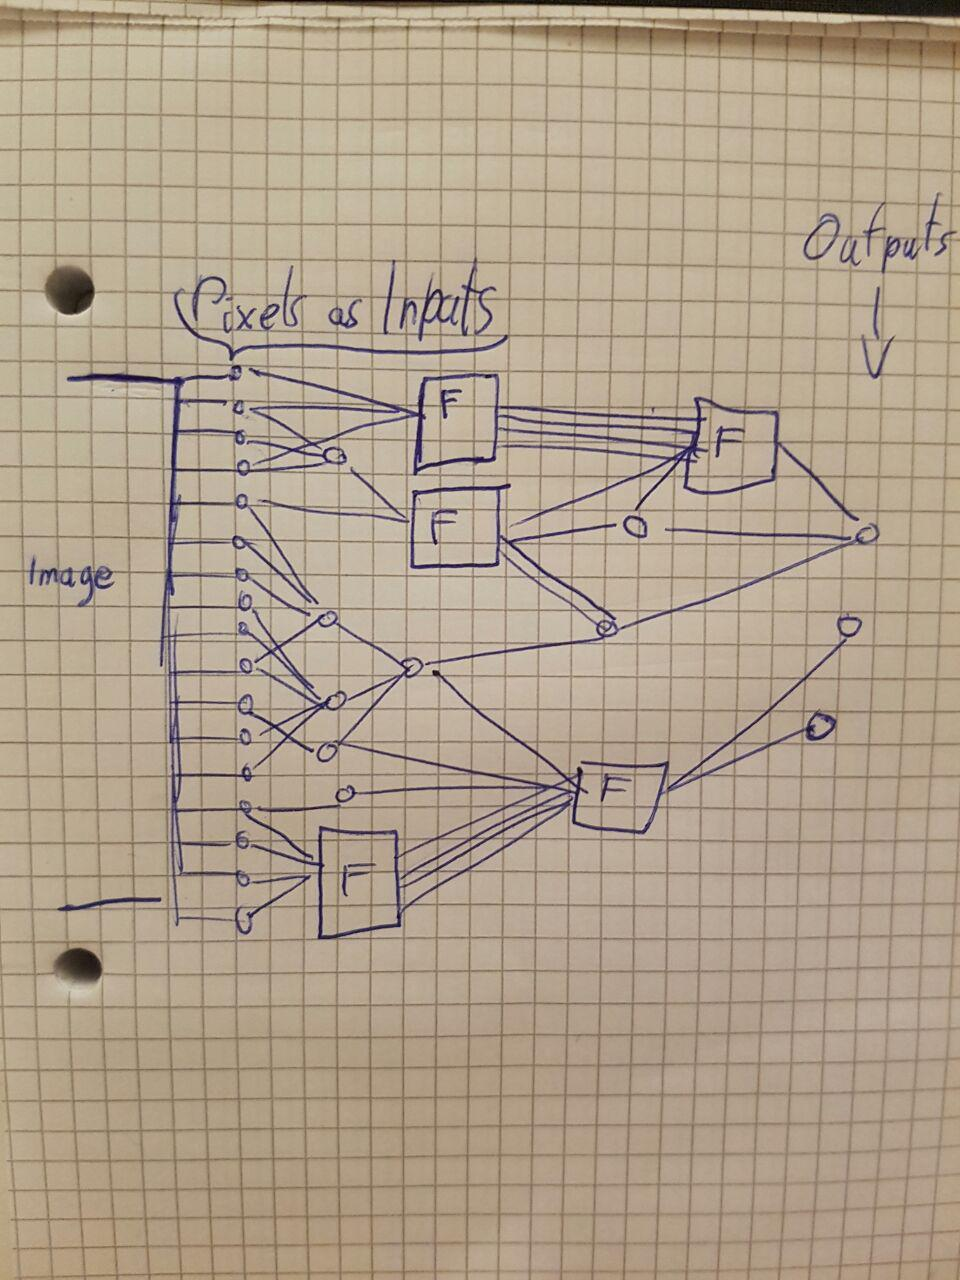
\includegraphics[scale=0.4]{approachone.jpg}  

This approach is probably as modular as it gets, however it brings various problems when combining.  
\begin{enumerate}
	\item{We ignore one of the main advantages on CNN: Being able to drastically lower the number of inputs through subsampling}
	\item{We don't use Pooling or ReLU layers}
	\item{The significance of a single classic neuron in such a system is questionable}
	\item{The filters in the same layer have to have some way of communicating to form a convolution}
	\item{Adding a new filter in a convolution conflicts with previous learned parameters}
\end{enumerate}

We can't address all of these conflicts in a satisfactory way, so we decided to go on to a next approach.\\
We adressed issue 3 by separating the whole network into a convolutional and a fully connected part. This allows us to take issue 1 by adding the concept of a \emph{minimal network}, inspired by NEAT’s practice of always starting with combining all inputs with all outputs.\\
In our case, the minimal network would incorporate some combination of convolution and pooling to reduce the input space. While the exact form of it is debatable, we think a good starting point is LeNet, as it proved itself to be flexible in its application. \cite{YannLeCun1998}\\
The overhauled version would start out like this:\\
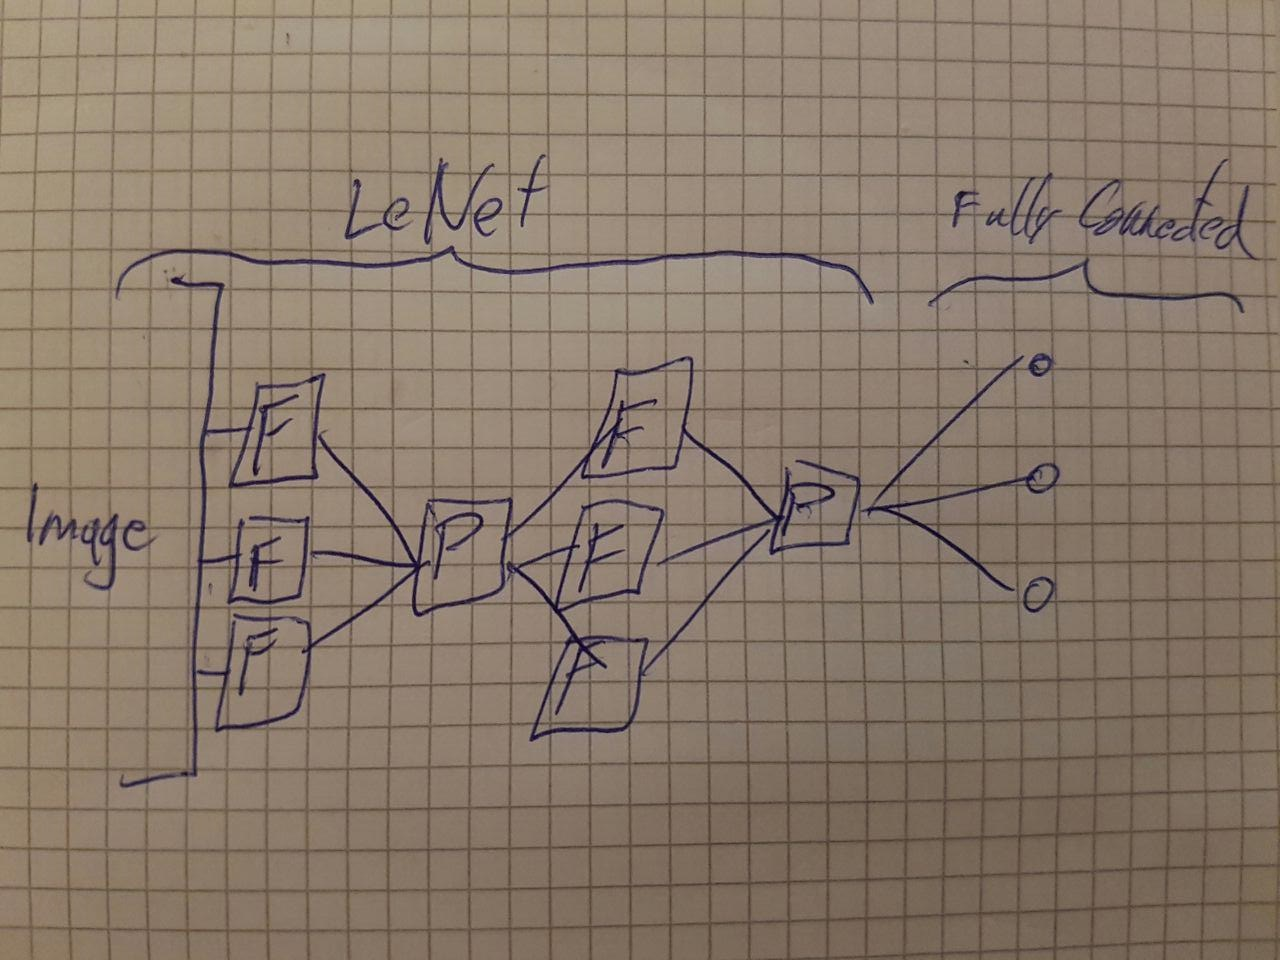
\includegraphics[scale=0.4]{approachtwoinit.jpg}\\
And could evolve into something like this:\\
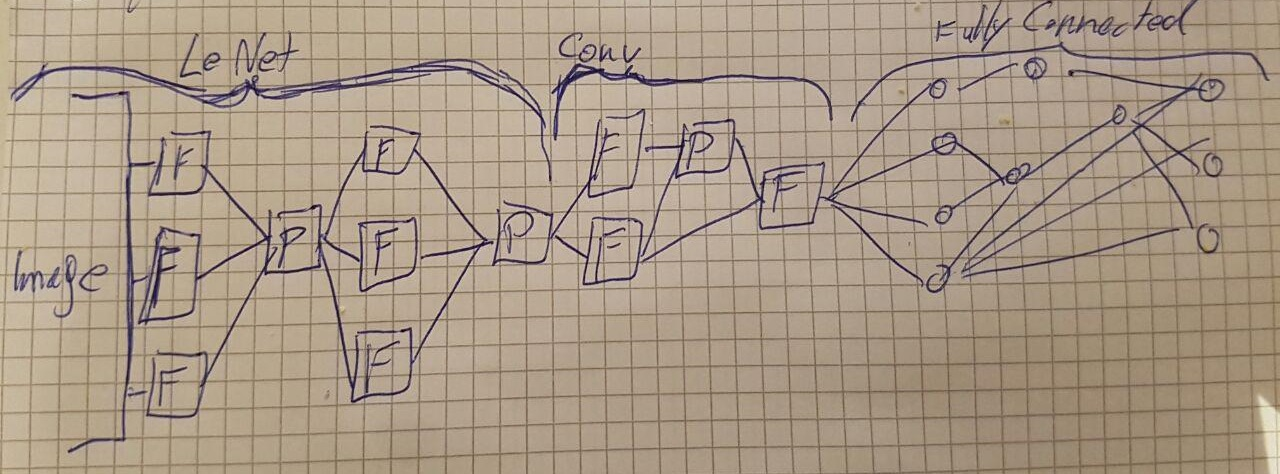
\includegraphics[scale=0.4]{approachtwoevolved.jpg}\\
This setup is problematic because filters are supposed to work together to form convolutions.\\
To process the same input (issue 4), the filters need to have the same size, which we cannot guarantee once we randomly insert new filters or, as per issue 2, pooling layers.\\
We can only scale the weight matrixes in the filters to the same size by either filling the smaller ones with a bunch of meaningless zeros or pooling the bigger one down, which, beeing a non-lossless compressing algorithm, makes our matrix less accurate.\\
We come to the conclusion that we have to limit the modularity of the Filters, as doing otherwise brings to many cons.  
Instead of letting the filters connect to whatever they want, we group them in convolutions.\\
These can alter the dimensionality of all filters in them at once, guaranteeing homogeneity and encapsulation.\\
With the filters now being synchronized in their convolutions, we have no more problems introducing poolers or ReLUs, as a convolution as a whole doesn’t care about the size of it’s input matrix.\\
Our updated pool of available units for stochastic insertion is now:  

\begin{table}[h]
	\begin{tabular}{ll}
		\textbf{Convolutional} & \textbf{Fully connected} \\
		Convolution            & Neuron                   \\
		Pooler                 &                          \\
		ReLU                   &                         
	\end{tabular}
\end{table}

Our starting topology now looks like this:\\
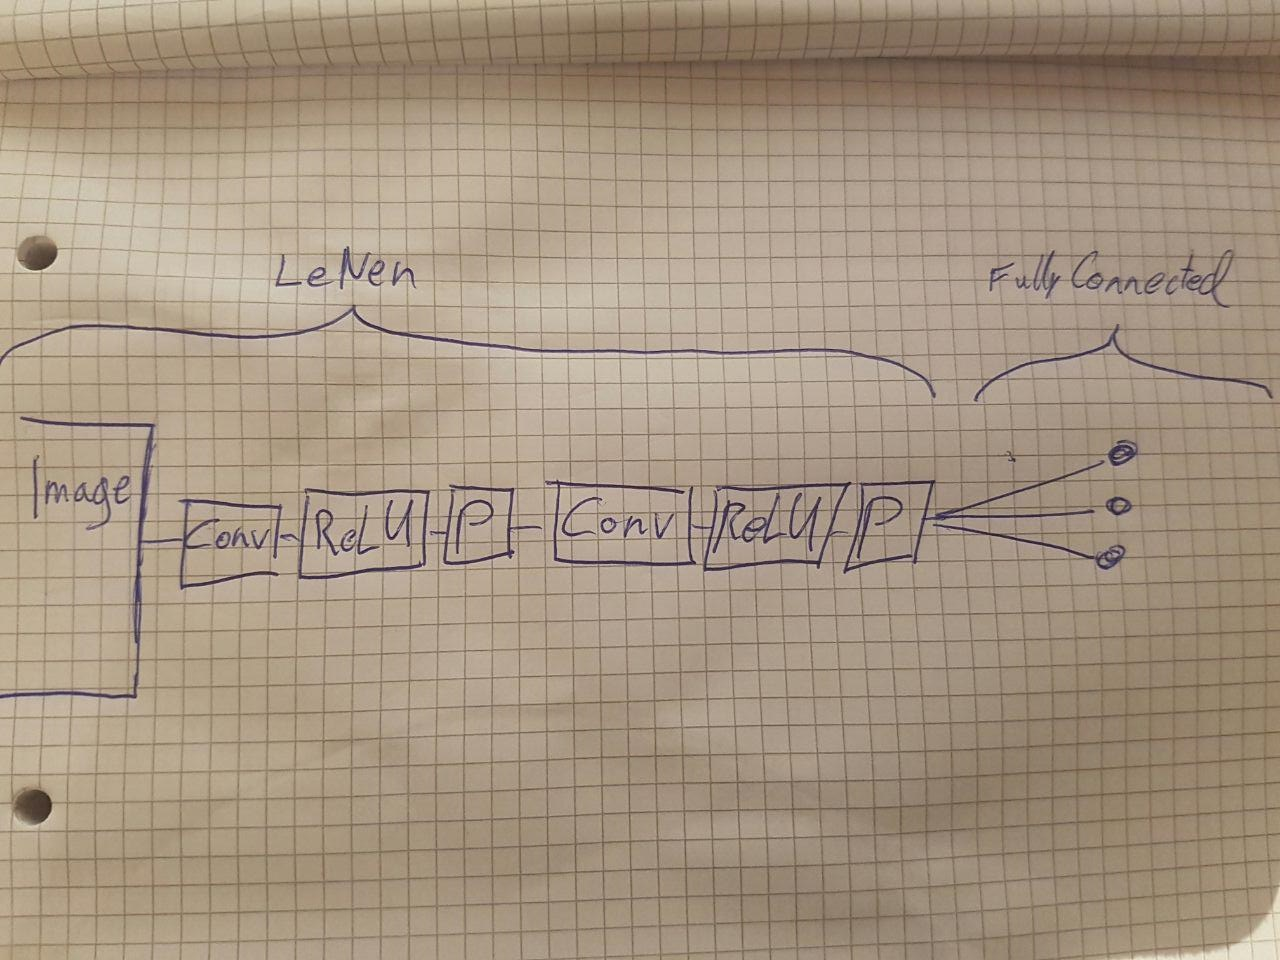
\includegraphics[scale=0.4]{approachthree.jpg}\\
The possible developments consist of a chain of random units right after LeNet.

This raises a new question: \emph{How is the meaning of the fully connected part altered when we add a new unit in the convolutional part?}\\
After detailed evaluation, we came to the conclusion that all of the parameters in the fully connected part would be fine tuned to a specific expected input. This expectation however ceases to be met once the dimensionality of the convolutions changes, as this shifts a lot of weight parameters towards a new meaning.\\
This means that we have two choices on how to process the fully connected part in case of a topological change in the convolutional part:
\begin{enumerate}
	\item{Adjust weights for the new meaning}
	\item{Trash the fully connected part and train it anew}
\end{enumerate}  
Both of these possibilities are not satisfactory. 1 will take a long time, since the already trained fully connected 4structure is basically meaningless now. 2 throws away big, otherwise perfectly usable, parts of the network.\\
After some research into this problem we found a recent paper from Google, describing how to get rid of the fully connected layer completely by using a global average pooler \cite{Lin2014}.\\
If we treat the feature map matrix \(F\) at the \(l\)th dimension as a vector \(F'_l\), the global average pooler is defined as follows:
\[ f(F'_l) = \frac{\sum_{i = 1}^{n} F'_{li}}{n} \]
We then forward the results of every layer to the softmax layer.\\
Provided the last layer of the convolutional part outputs a tensor with exactly as many dimensions as the number of possible network output, we can exchange the complete fully connected part for this global average pooler while achieving the same results with a drastically improved performance in both evaluation and search space. \cite{Lin2014}\\
The reason is, in a nutshell, that we stop imagining the output of a filter as detection of a feature.\\
We now treat it as a rate of confidence: The bigger the numbers, the more confident we are that the feature is present.\\
This means that the feature detection is no longer performed by the fully connected part, but instead by every single filter in the network together \cite{Lin2014}.
Our standard network now looks like this:\\
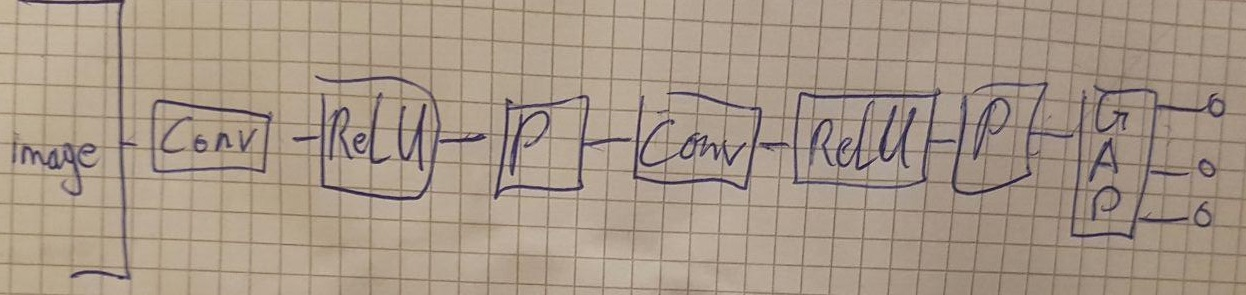
\includegraphics[scale=0.4]{approachfour.jpg}\\

And could develop into something like this:\\
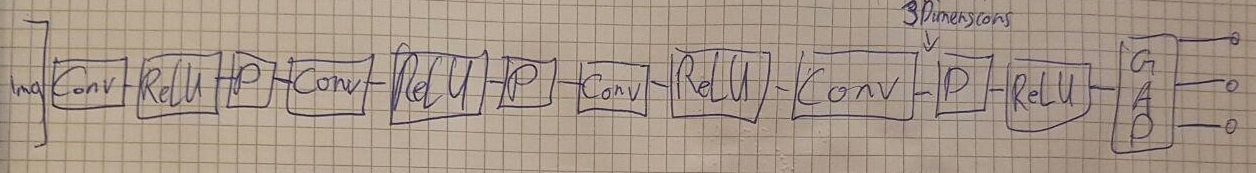
\includegraphics[scale=0.4]{approachfourevol.jpg}\\

We now seem to have resolved all issues, however when looking at the layers of the example, we see that it has a depth of 8 logical layers (ReLU layers are not counted because they do not result in a feature extraction, as they are merely activation functions). This huge amount is very atypical and has been shown to result is various problems such as very high hardware requirements and lower accuracies\cite{Simonyan2015}.\\
The fundamental problem is that the effect of a change in the parameters in a lower layer becomes abysmal compared to a change in the higher ones \cite{Simonyan2015} \cite{Hochreiter1991}.
A network of this size is not realistically trainable by us. 

A very recent paper now belonging to the Facebook AI Research group deals with these issues.\\
They introduce the concept of Residual Networks, in short ResNets. \cite{KaimingHe2015}\\
Their goal was to create a convolutional network by combining an arbitrary amount of well defined residual units on which these problems are of no concern.
Overly simplified, they address the problem of varying influence by adding a new kind of connecting, called a shortcut.\\

What it does is simply add matrixes. If they have different dimensionalities, the smaller matrix gets projected on the bigger one by being processed by a one by one matrix with a respective number of filters.\\

A residual block looks like this: \\
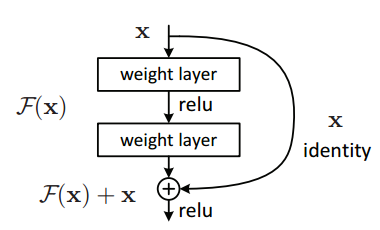
\includegraphics{shortcut.PNG}\\
On the left side, a convolutional action takes place (in this case two convolutions with one ReLU activation inbetween). On the right side, the original input of the residual block is added to its output.\\
This overlay guarantees that the convolutions cannot alter the original state too much, as they now merely highlight features as opposed to extracting them.\\
The issue of performance is addressed by applying a bottleneck.\\
This means downsampling the input dimensionality of the residual block by applying one by one convolutions before performing the convolution and then upscaling it again. This procedure is inspired by Googles Network In Network Inception structure \cite{KaimingHe2015} \cite{Lin2014}.\\
The overhauled residual block now looks like this:\\
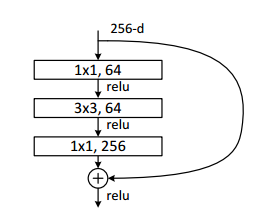
\includegraphics{bottleneck.PNG}\\
While more convolutions would in theory be possible, only one is used, as the bottleneck dimension poolers introduce new parameters themselves.\\
This method has been demonstrated to achieve very similar levels of accuracy while reducing a bit chunk of the computational cost \cite{KaimingHe2015}.\\
Residual Blocks are modular by nature, so they are a perfect fit for our NEAT algorithm. When analyzing them, we can easily extract following parameters from them:\\
\begin{enumerate}
	\item{Weights of first dimension pooler}
	\item{Weights of convolution pooler}
	\item{Weights of second dimension pooler}
	\item{Downscaled number of dimensiona}
	\item{Upscaled number of dimensiona}
	\item{Number of convolutions}
\end{enumerate}